\section{Method}
\label{sec:method}
    % \begin{figure*}[htb]
    %     \centering
    %     
\includegraphics[width=0.8\linewidth]{images/homotopy.png}
    %     \caption{A cartoon illustration of our homotopy-based strategy on a single camera. We simulate a virtual problem with associated system $\mathcal{S}_0$ for which we know all the parameters and the solutions. These are evolved to the real system $\mathcal{S}_1$ that correspond to the actual calibration and localization problem at hand.}
    %     \label{fig:homotopy}
    % \end{figure*}
By collecting the pairs of geometric constraints associated with each visible silhouette line $l^h_{ij}$ across all images, we obtain a system of polynomial equations of the form~\eqref{eq:dual_quadric_constraint} and \eqref{eq:vertex_constraint}. We refer to this as the \emph{original system} $\mathcal{S}_1$, as it encodes the multi-view geometric relationships between the known 3D scene and the actual, but unknown, camera matrices $\PP_i = \KK[\RR_i, \mathbf{t}_i]$. Solving $\mathcal{S}_1$ directly is  challenging due to its high degree, multiple spurious solutions, and the presence of non-linearities.
To overcome these challenges, we design a custom homotopy based on silhouette lines. We begin by constructing a \emph{synthetic}, geometrically consistent starting system $\mathcal{S}_0$, which collects the constraints between the 3D cylinders and a set of silhouette lines generated by known synthetic cameras. 
As sketched in Figure~\ref{fig:homotopy}, at high level, we  continuously deform $\mathcal{S}_0$ into the target real system $\mathcal{S}_1$ through a homotopy parametrized by $t \in [0,1]$, gradually transforming the synthetic silhouette lines into the observed ones in a geometric consistent way, while tracking the corresponding camera parameters, denoted by $\mathbf{x}(t)$, throughout the process. At $t = 0$, the solution $\mathbf{x}(0)$  of $\mathcal{S}_0$ corresponds to the known synthetic cameras, whereas the tracked solution at $\mathbf{x}(1)$ yields the estimated cameras configuration that solves the real original problem.

\subsection{The original target system $\mathcal{S}_1$}
Let $\mathcal{L}_1$ denote the collection of all visible silhouette lines from all cylinders across all images. Each visible silhouette line $l_{ij}^h \in \mathcal{L}_1$ contributes two quartic equations, given by ~\eqref{eq:dual_quadric_constraint} and~\eqref{eq:vertex_constraint}, which together define the original system $\mathcal{S}_1$. With a slight abuse of notation, since the set of silhouette lines $\mathcal{L}_1$ defines the parameters of the system, we can write $\mathcal{S}_1(\mathbf{x},\mathcal{L}_1)$ to emphasize this dependency.
As observed in \cite{gummeson24relative},  \eqref{eq:vertex_constraint} involves only the intrinsic $\KK$ and the rotation $\RR$. For a cylinder $\mathcal{C}_j$ captured in the $i$-th image $I_i$ by a camera $\PP_i=\KK[\RR_i,\mathbf{t}_i]$ we have
 \begin{equation}
             l^{h\top}_{ij} \KK [\RR_i|\mathbf{t}_i] \ \begin{pmatrix}
                \mathbf{w}_j \\
                0
            \end{pmatrix} = l^{h\top}_{ij} \KK\RR \mathbf{w}_j
             = 0.
    \label{eq:expanded_vertex_constraint}
    \end{equation}
Thus, one could solve for $\KK$ and all $\RR_i$ from all the equations in $\mathcal{S}_1$ of the form \eqref{eq:vertex_constraint}. Then from all the equations of the form \eqref{eq:dual_quadric_constraint}, solve for the translations $\mathbf{t}_i$.

Using this approach, assuming $V$ visible silhouette lines in total, the system $\mathcal{S}_1$ contains $V$ equations of the type~\eqref{eq:vertex_constraint}.  The number of unknowns is $3N + 5$, corresponding to the 3 rotation parameters per view and the 5 intrinsic parameters of the camera. Therefore, solving for the camera intrinsics and all rotations requires satisfying the inequality:
\begin{equation}
V \geq 3N + 5.
\end{equation}
Once $\KK$ and the rotations $\RR_i$ are estimated, the translations $\mathbf{t}_i$ can be recovered from the remaining $V$ equations of  type~\eqref{eq:dual_quadric_constraint}, which are quadratic in $\mathbf{t}_i$.

In practice, given $M$ cylinders, under the assumption of full visibility (\emph{i.e.}, $V = 2MN$ silhouette lines), $\mathcal{S}_1$ can be solved if

\begin{equation}
      \begin{aligned}
              2NM \ge 3N + U \\
              M \ge \ceil*{\frac{3}{2} + \frac{U}{2N}}
      \end{aligned}
      \label{eq:SolvableConditionSimple}
\end{equation}

for each $(M,N)$ pair feasibility is reported in Table~\ref{tab:scene_configurations}.
A single cylinder  $M=1$ does not allow for  solution, while beyond $M=6$ or $N=9$, $\mathcal{S}_1$ is always solvable. 

\subsection{The synthetic starting system \texorpdfstring{$\mathcal{S}_0$}{S0}}
\label{sec:synthetic_system}

To construct the synthetic system $\mathcal{S}_0$, we begin by generating a set of $N$ synthetic cameras, denoted $\{\PP_i^{(0)} = \KK^{(0)}[\RR_i^{(0)}\,|\,\mathbf{t}_i^{(0)}]\}$, where both the intrinsic parameters $\KK^{(0)}$ and the extrinsic parameters $(\RR_i^{(0)}, \mathbf{t}_i^{(0)})$ are known. Given the 3D structure of the scene (\emph{i.e.}, the known cylinders), we project them into each synthetic view to compute the corresponding silhouette lines $\mathcal{L}_0 = \{l^{h(0)}_{ij}\}$.

These silhouette lines are then used to construct equations that contain constraints such as~\eqref{eq:dual_quadric_constraint} and~\eqref{eq:vertex_constraint}. Mimicking what we have done for the orginal system $\mathcal{S}_1$, by collecting all such equations for each visible silhouette in the synthetic setup, we define the system $\mathcal{S}_0(\mathbf{x},\mathcal{L}_0)$. This system is guaranteed to be consistent by construction, and its solution $\mathbf{x}(0)$ corresponds exactly to the known parameters of the synthetic camera  used to generate it.


\subsection{Custom silhouette-based homotopy}
\label{sec:silhouette-based-homotopy}

To solve $\mathcal{S}_1(\mathbf{x},\mathcal{L}_1)$ we will use a parametric homotopy, as explained in Section\ref{sec:parametric_homotopy} a parametric homotopy~\cite{may2004parametrizedhomotopytheory} is a specialization of the general homotopy framework in which the structure of the system and the family of equations remains fixed, while the parameters defining such instance of our family vary continuously. In our case, since the 3D cylinders are fixed they are treated as part of the family definition as constants, silhouette lines position in each image are our parameters defining the specific instance and the camera parameters $\KK$ and $RR_i$ for each view are the unknown. The key idea is to continuously transform over time $t$ the silhouette lines to interpolate between those generated synthetically in $\mathcal{S}_0$ and those observed in the real system $\mathcal{S}_1$.

The effectiveness of each path tracking depends on the ability to continuously deform the synthetic silhouette lines into the observed ones, while maintaining the geometric constraints imposed by the cylinders. This is crucial to ensure that the homotopy remains well-defined and converges to a solution that respects the original geometric relationships.

To this end, we developed a custom homotopy function that apply to each silhouette line a transformation $T(t; \mathcal{L}_0, \mathcal{L}_1)$, as illustrated in Figure~\ref{fig:transformation}. Given a synthetic line $l^{h(0)}_{ij} \in \mathcal{L}_0$ and its corresponding observed line $l^{h}_{ij} \in \mathcal{L}_1$, the transformation $T(t; \mathcal{L}_0, \mathcal{L}_1)$ rotates the synthetic line around the intersection point $O= l^{h(0)}_{ij} \times l^{h}_{ij}$ by an angle $\theta(t) = t\alpha$, where $\alpha$ is the angle between the two lines. At $t = 0$, the synthetic line remains unchanged; at $t = 1$, it fully aligns with the observed line. Formally $T(t; \mathcal{L}_0, \mathcal{L}_1)$ is a transformation matrix defined as follows:

\begin{equation}
T(t; \mathcal{L}_0, \mathcal{L}_1) =
    \begin{bmatrix}
    \cos(\theta(t)) & -\sin(\theta(t)) & -O_x \cos(\theta(t)) + O_y \sin(\theta(t)) + O_x \\
    \sin(\theta(t)) & \cos(\theta(t)) & -O_x \sin(\theta(t)) - O_y \cos(\theta(t)) + O_y \\
    0 & 0 & 1
    \end{bmatrix}
\end{equation}

\begin{figure}
\centering
  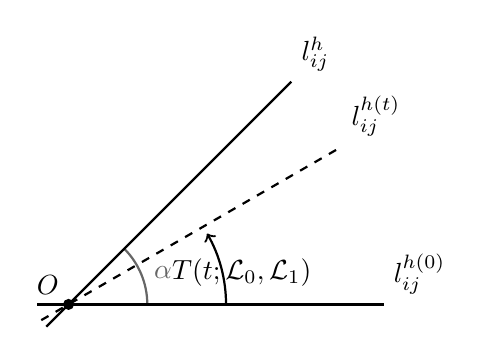
\begin{tikzpicture}[scale=2.0]
            % Define origin
            \coordinate (O) at (0,0);
            
            % Define directions
            \coordinate (A) at (2,0);        % l^{h(0)}_{ij}
            \coordinate (B) at ({2*cos(30)}, {2*sin(30)});  % l^{h(t)}_{ij}
            \coordinate (C) at ({2*cos(45)}, {2*sin(45)});  % l^{h}_{ij}
            \coordinate (AS) at (-0.2, 0);
            \coordinate (BS) at ({0.2*cos(210)}, {0.2*sin(210)});
            \coordinate (CS) at ({0.2*cos(225)}, {0.2*sin(225)});
            
            % Draw lines
            \draw[thick] (AS) -- (A) node[above right] {$l^{h(0)}_{ij}$};
            \draw[thick, dashed] (BS) -- (B) node[above right] {$l^{h(t)}_{ij}$};
            \draw[thick] (CS) -- (C) node[above right] {$l^h_{ij}$};
            
            % Mark point O
            \fill (O) circle (1pt) node[above left] {$O$};
            
            % Draw angles
            \draw[->, thick] (1.0,0.0) arc[start angle=0, end angle=30, radius=0.9cm];
            \node at (1.1,0.2) {$T(t; \mathcal{L}_0, \mathcal{L}_1)$};
            
            \draw[-, thick, opacity=0.6] (0.5, 0.0) arc[start angle=0, end angle=45, radius=0.5cm];
            \node[opacity=0.6] at (0.6,0.2) {$\alpha$};
        \end{tikzpicture}
        \caption{The rotation $T(t; \mathcal{L}_0, \mathcal{L}_1)$ continuously transforms the synthetic lines $l^{h(0)}_{ij}$ towards the observed lines $l^{h}_{ij}$ by applying a rotation of an angle $t\alpha$ around the intersection point $O$. At the end of the homotopy, $T(t; \mathcal{L}_0, \mathcal{L}_1)$  transforms the synthetic parameters $\mathcal{L}_0$ of our problem to the observed parameters $\mathcal{L}_1$.}\label{fig:transformation}
\end{figure}

With a slight abuse of notation, we denote by $T(t; \mathcal{L}_0, \mathcal{L}_1)\mathcal{L}_0$ the set of silhouette lines obtained by applying the transformation $T(t; \mathcal{L}_0, \mathcal{L}_1)$ to the synthetic lines in $\mathcal{L}_0$. Our silhouette-based parametric homotopy can then be compactly written as:
\begin{equation}
    H(\mathbf{x}(t), t) := \mathcal{S}_t(\mathbf{x}(t), T(t; \mathcal{L}_0, \mathcal{L}_1)\mathcal{L}_0),
    \label{eq:LineCameraHomotopy}
\end{equation}
where $\mathbf{x}(t)$ represents the set of camera parameters being tracked (namely intrinsics $\KK$ and rotations $RR_i$ for each view), and $\mathcal{S}_t$ is the system whose structure remains fixed, while the parameters $T(t; \mathcal{L}_0, \mathcal{L}_1)\mathcal{L}_0$ (the transformed silhouette lines) evolve from synthetic to real.

This, in turn, is solved using Julia homotopy continuation package~\cite{HomotopyContinuationJL} with an implementation of the ad-hoc homotopy described above.

Each solution is substituted in~\eqref{eq:dual_quadric_constraint}. Since the resulting equation in $\mathbf{t}$ is quadratic, we decided to solve it directly using a total degree homotopy. The attained solutions are first filtered based on geometric properties \eg{cameras that are not looking at the provided cylinders}, and then evaluated using reprojection error to pick the best performing one.

\subsection{Iterating the procedure}
\label{sec:iterating_procedure}

Convergence to the real solution, while not violating the system constraints, is not always garaunteed. For this reason if the process for a starting \emph{synthetic} system $\mathcal{S}_0$ is halted prematurely by the homotopy package the process is repeated for a new system $\mathcal{S}_0$ by drawing a new set of \emph{synthetic} cameras.

Homotopy continuation is garaunteed to find a solution if the number of paths explored $p$ is at least equal to the number of solutions of the system.
If the number of paths explored $p$ is the same as the number of solutions $n^d$ of the system, then the homotopy is said to be \emph{optimal}~\cite{HomotophyContinuationMethods}. But constructing optimal homotopies is in general so far not possible. We don't even know an efficient method to compute the number of solutions of for a polynomial system $F(x)$. Intersection theory (a part of algebraic geometry) \cite{khovanskii2011faa4} allows to compute this in theory, but proving the number of solutions even for one particular polynomial system is usually unfeasible.
A theorem of algebraic geometry~\cite{HomotophyContinuationMethods} states that the number of solutions of a polynomial system is bounded by the number of solutions of the start system. Since \emph{total degree homotopies} always converges the number of paths cannot be greater that the number of solutions of the \emph{total degree homotopy} associated with our system. A total degree homotopy system of $f = (f_1, f_2, \ldots, f_p)$ of degree $d_1, d_2, \ldots, d_p$ has at most $d_1 \cdot d_2 \ldots \cdot d_p$ solutions, where $d_i$ is the degree of the polynomial $f_i$. In our case, since we are dealing with quartic equations, the number of solutions is at most $4^{3N + 5}$ for a full calibration.

For the full camera calibration, using this method, on average $177147$ paths (initial solutions) are tracked and $64$ possible solutions are found, for the most common skew$=0$ case $59049$ paths are tracked and $112$ solutions are found, and finally to localize a calibrated camera $64$ paths and $16$ solutions.

We will now go through the different steps we took to optimize the number of trials, namely: intrinsic initialization, poses initialization, lines generation, monodromy, best practices on iterating the procedure.

Algorithm~\ref{alg:solutions_generation} summarizes the procedure and a graphical representation is available in Figure~\ref{fig:homotopy}.

\paragraph{Intrinsics initialization}
If avaible a priory knowledge about the scene can be leveraged, \eg{we know the model of the camera and it's specifications but want to account for manufacturing flactuations}. If no prior about focal length is known, assuming a square focal length of value $2000$ is a reasonable guess for a smartphone camera (line 1). Principal point is initialized at $c_x = IMAGE\_WIDTH / 2, \; cy = IMAGE\_HEIGHT / 2$ (line 2). The skew parameter is set to a small value different from $0$ (line 3).

\paragraph{Poses initialization}
For the first camera position $\mathbf{t}_0^{(1)}$ randomizing three unitary values for the direction and multiplying such resulting vector by a constant scale factor (line 7) gives the most freedom.
Guessing the metric scale of the scene and using it as the scale makes testing and validating results easier but if it's not possible any random value will yield the same quality results.
For every other camera Algorithm~\ref{alg:next_camera_pose} is used. A random offset unit vector $\mathbf{f}_i$ (line 1), and a distance $d_i = N(|\mathbf{t}_0^{(0)}|, \frac{|\mathbf{t}_0^{(0)}|}{v})$ (line 2) are drawn. The parameter $v$ can be tweaked depending on the apparent camera movement between shots. Closer shots higher values of $v$.

\begin{equation}
    \mathbf{t}_0^{(n)} = \mathbf{t}_0^{(n-1)} + d_i\mathbf{f}_i
\end{equation}

Rotation $\RR_i$ for each camera is picked with a \emph{look at} function pointed at the world origin $\mathbf{o} = \left[N(0, \sigma), N(0, \sigma), N(0, \sigma) \right]$ (line 4) where $\sigma$ can be tweaked depending on the scene scale.

\begin{algorithm}
\caption{next\_camera\_pose}
\label{alg:next_camera_pose}
    \begin{algorithmic}[1]
        \REQUIRE $\mathbf{t}_0^{(i-1)}$
        \STATE $\mathbf{f}_i \gets \var{normalize}(\var{random}(3))$
        \STATE $d_i \gets N(|\mathbf{t}_0^{(i-1)}|, \frac{|\mathbf{t}_0^{(i-1)}|}{v})$ \; \; (random distance)
        \STATE $\mathbf{t}_0^{(i)} \gets \mathbf{t}_0^{(i-1)} + d_i \mathbf{f}_i$
        \STATE $\RR_0^{(i)} \gets \var{look\_at}(\var{world\_origin})$
        \RETURN $\mathbf{t}_0^{(i)}, \RR_0^{(i)}$
    \end{algorithmic}
\end{algorithm}

This is used in Algorithm~\ref{alg:solutions_generation} (lines 8-10) to initialize the camera poses $\mathbf{t}_0^{(i)}$ and $\RR_0^{(i)}$ for each camera $i$.

\paragraph{Lines generation}
For each camera $i$ the projection matrix $\PP_0^{(i)}$ is constructed as (line 14):
\begin{equation}
    \PP_0^{(i)} = \KK_0^{(i)} \left[\RR_0^{(i)} \;|\; \mathbf{t}_0^{(i)}\right]
\end{equation}
Collecting the set of all projection matrices makes up the initial solution $\mathbf{x}_0$ (line 19).
We can use it to project each cylinder $C_j$ onto it's silhouette lines $l_{ij}^{h}, \; h=1,2$ through Algorithm~\ref{alg:get_cylinder_contours} (line 15).

The silhouette lines $l_{ij}^{h(0)}$ are collected and used to construct the parameters $\mathcal{L}_0$ (line 18).
$\mathbf{x_0}$ together with the set of silhouette lines $\mathcal{L}_0$ make up the synthetic system $\mathcal{S}_0$.

\paragraph{Monodromy}
Right now we only have one solution for the set of lines $\mathcal{L}_0$. To increase the success rate of our homotopy we run our synthetic solution $\mathbf{x}0$ through a Monodromy~\ref{sec:monodromy} (line 20). A monodromy starts from a solution and through random walking in the complex space $\mathbb{C}$ generates new, mostly complex, solutions for our problem. This increases the number of paths that we can follow which improves convergence significantly. The number of new solutions found depends on the number of intrinsic parameters to estimate. For the full calibration case it's no less than $32$ and usually it's $64$.

\paragraph{Applying homotopy continuation}
For each solution $\mathbf{x}_0^{(w)}$ of the monodromy $\mathcal{X}_0$, we apply homotopy continuation using the silhouette-based homotopy function $H$ defined in~\eqref{sec:silhouette-based-homotopy} (line 22). The homotopy package returns a set of solutions $\var{solutions}$, which are then iterated over (line 23).
For each solution $\mathbf{x}_1$ of $\var{solutions}$, we extract the intrinsic parameters $\mathbf{K}_1$ (line 24), rotation matrices $\RR_1^{(i)}$ (line 26), and apply a total degree homotopy to estimate each camera translation $\mathbf{t}_1^{(i)}$ (line 27).

Finally, we compute the reprojection error for each solution (line 29) and keep track of the best solution found so far (lines 30-33). The best solution is returned at the end of the procedure (line 37).

\paragraph{Iterating the procedure}
If the homotopy is halted by the framework and we never reach the end of the current iteration (line 45) we repeat the process discarding the first camera pose and shifting each one to the left (line 39-42). A new camera $N$th camera pose is generated with Algorithm~\ref{alg:next_camera_pose} (line 43). This garauntees that new iterations will be evenly spaced with respect to most of the previous ones.

% Algorithm: Solution Generation and Homotopy Procedure
\begin{algorithm}[H]
\caption{Solution Generation and Homotopy Procedure}
\label{alg:solutions_generation}
\begin{algorithmic}[1]
\REQUIRE Scene geometry (cylinders), observed silhouette lines $\mathcal{L}_1$, number of cameras $N$
\STATE $f_x \gets 2000$, $f_y \gets 2000$
\STATE $c_x \gets W_{image}/2, c_y \gets H_{image}/2$
\STATE $s \gets 0.01$
\STATE $\KK_0 \gets \left[
                \left[ f_x\; s \; c_x \right],
                \left[ 0 \; f_y \; c_y \right],
                \left[ 0 \; 0 \; 1 \right]
            \right]$ \; \; (initial intrinsic parameters)
\STATE $\var{best\_solution} \gets \var{null}$
\STATE $\var{best\_error} \gets \infty$
\STATE $\mathbf{t}_0^{(1)} \gets \var{random}(3) * SCALE$
\FOR{$i = 2$ to $N$}
    \STATE $\mathbf{t}_0^{(i)}, \RR_0^{(i)} \gets \var{next\_camera\_pose}(\mathbf{t}_0^{(i-1)})$ \; \; (see Algorithm~\ref{alg:next_camera_pose})
\ENDFOR
\FOR{$z = 1$ to $Z$}
    \FOR{each camera $i$}
        \FOR{each cylinder $\CC_j$}
            \STATE $\PP_0^{(i)} \gets \KK_0^{(i)} [\RR_0^{(i)}\,|\,\mathbf{t}_0^{(i)}]$ \; \; (projection matrix)
            \STATE $l_{ij}^{h(0)} \gets \var{get\_cylinder\_contours}(\CC_j, \PP_0^{(i)})$ \; \; (see Algorithm~\ref{alg:get_cylinder_contours})
        \ENDFOR
    \ENDFOR
    \STATE $\mathcal{L}_0 \gets \left\{ l_{ij}^{h(0)} \mid i=1,\ldots,N, j=1,\ldots,M, h=1,2 \right\}$ \; \; (synthetic silhouette lines)
    \STATE $\mathbf{x}_0 \gets \left[\KK_0, \RR_0^{(1)}, \ldots, \RR_0^{(N)}, \mathbf{t}_0^{(1)}, \ldots, \mathbf{t}_0^{(N)}\right]$ \; \; (initial solution)
    \STATE $\mathcal{X}_0 \gets \var{monodromy}(\mathcal{S}_0, \mathbf{x}_0, \mathcal{L}_0)$ \; \; (generate new solutions)
    \FOR{each solution $\mathbf{x}_0^{(w)}$ of $\mathcal{X}_0$}
        \STATE $\var{solutions} \gets \var{homotopy}_H(\mathcal{S}_0 \mathbf{x}_0^{(w)}, \mathcal{L}_0)$ \; \; (apply homotopy function $H$ defined in~\eqref{sec:silhouette-based-homotopy})
        \FOR{each $\mathbf{x}_1$ of $\var{solutions}$}
            \STATE $\mathbf{K}_1 \gets \mathbf{x}_1^\KK$
            \FOR{each camera $i$}
                \STATE $\RR_1^{(i)} \gets \mathbf{x}_1^{\RR_i}$
                \STATE $\mathbf{t}_1^{(i)} \var{homotopy}_{\var{total\_degree}}(\mathcal{L}_1)$ \; \; (total degree homotopy does not require start solutions)
            \ENDFOR
            \STATE $\var{error} \gets \var{reprojection\_error}(\mathcal{S}_1, \mathbf{x}_1, \mathcal{L}_1)$ \; \; (compute reprojection error)
            \IF{$\var{error} < \var{best\_error}$}
                \STATE $\var{best\_solution} \gets \mathbf{x}_1$
                \STATE $\var{best\_error} \gets \var{error}$
            \ENDIF
        \ENDFOR
    \ENDFOR
    \IF{$\var{homotopy\_halted}$}
        \STATE $\var{best\_solution} \gets \var{null}$ \; \; (reset best solution)
        \STATE $\var{best\_error} \gets \infty$ \; \; (reset best error)
        \FOR{$i = 1$ to $N-1$}
            \STATE $\mathbf{t}_0^{(i)} \gets \mathbf{t}_0^{(i+1)}$ \; \;
            \STATE $\RR_0^{(i)} \gets \RR_0^{(i+1)}$ \; \;
        \ENDFOR
        \STATE $\mathbf{t}_0^{(N)}, \RR_0^{(N)} \gets \var{next\_camera\_pose}(\mathbf{t}_0^{(N-1)})$ \; \; (see Algorithm~\ref{alg:next_camera_pose})
    \ELSE
        \RETURN $\var{best\_solution}$
    \ENDIF
\ENDFOR
\end{algorithmic}
\end{algorithm}

\subsection{Handling spurious solutions}
\label{sec:postprocessing}
Homotopy continuation methods do not allow to force inequality constraints, and as a result, the solver may converge to solutions that are not physically valid, namely a negative focal length or negative skew. To address this issue, we introduce a novel correction step that exploits the fact that the calibration matrix $\KK$ and the rotation matrix $\RR$ appear as a product in~\eqref{eq:expanded_vertex_constraint}. Specifically, if $(\KK, \RR)$ is a solution to~\eqref{eq:expanded_vertex_constraint}, then for any invertible matrix $\CC$, the pair $(\KK\CC, \CC^{-1}\RR)$ is also a valid solution, since:
\begin{equation}
    l^{h\top}_{ij} \KK \CC \CC^{-1}\RR \mathbf{w}_j = l^{h\top}_{ij} \KK \RR \mathbf{w}_j=0.
\end{equation}
Based on this observation, we propose to post-correct physically invalid solutions by designing a suitable correction matrix $\CC$ to enforce  positive focal length and skew.
A correction is valid if it does not change the absolute values of the intrinsic parameters and if $\CC^{-1}\RR$ is still a rotation, namely has unitary determinant and is orthogonal:
\begin{equation}
\begin{cases}
  \det(\CC^{-1}\RR) = \det(\CC^{-1})\det(\RR) = \det(\CC^{-1}) = \pm 1\\
   (\CC^{-1}\RR) (\CC^{-1}\RR)^\top = \CC^{-1}\RR\RR^\top\CC^{-\top} = \CC^{-1}\CC^{-\top} = \II.
  \end{cases}
\end{equation}
Since $\RR$ is a rotation matrix, it is orthogonal and already satisfies both properties allowing for the substitutions made.
Note that we allow $\det(\CC)=-1$ because  a reflection might actually be needed to make the solution geometrically consistent. 

Using this property, we derive three corrections $\CC_{f_x},\CC_{f_y},\CC_{sf_y}  $
\begin{equation}
  \CC_{f_x} = \begin{pmatrix}
                -1 & 0 & 0 \\
                0 & 1 & 0 \\
                0 & 0 & 1
            \end{pmatrix}, \quad 
                   \CC_{f_y} = \begin{pmatrix}
                1 & \frac{2\alpha}{f_x} & 0 \\
                0 & -1 & 0 \\
                0 & 0 & 1
            \end{pmatrix}, \quad 
                     \CC_{s f_y} = \begin{pmatrix}
                1 & 0 & 0 \\
                0 & -1 & 0 \\
                0 & 0 & 1
            \end{pmatrix},
\end{equation}
to correct $f_x, f_y$ and, the skew $s$ and $f_y$ jointly respectively.

Note that multiple corrections $\CC_1$, $\CC_2$ can be applied to the same solution $(\KK,\RR)$ by nesting them into one another
\begin{equation}
    \KK \CC_1 \CC_2 \CC_2^{-1} \CC_1^{-1}\RR = \KK' \CC_2 \CC_2^{-1} \RR'
\end{equation}
Since $\KK', \RR'$ still satisfy all the constraints above.

Unfortunately, we can not find a rotation $\CC_s$ to correct the skew alone.
